\documentclass[paper=a4,11pt,german]{scrartcl} % default ist 10pt (zu klein)

\usepackage[utf8]{inputenc} % dokument muss dann auch als UTF-8 (ohne BOM) gespeichert werden
\usepackage[ngerman]{babel}

% schrfitauswahl
\usepackage[T1]{fontenc}
\usepackage[sc]{mathpazo}  % alternativ \usepackage{charter}
%\linespread{1.05}
\usepackage[scaled]{beramono}
\usepackage{multicol}
\setkomafont{sectioning}{\normalcolor\bfseries} % Ändert Überschriftschriftart (nun mit Serifen)

\usepackage{graphicx} 
% als letztes package (fuer funktionierende Link im und ausserhalb des Dokuments)
\usepackage[pdftex]{hyperref} 

% ggf. falsche Worttrennung hier korrigieren
\hyphenation{op-tical net-works semi-conduc-tor Grund-idee}

\begin{document}
%
% paper title
% can use linebreaks \\ within to get better formatting as desired
\title{Asymmetrische Kryptographie in Java}

\author{Norman Vetter\\
\textbf{Seminar "`Sichere verteilte Anwendungen mit Java"'}\\
Universität Potsdam\\
Wintersemester 2012/13}

\date{}

% make the title area
\maketitle

% Nicht bei einer Seminarausarbeitung. Da reicht die Zusammenfassung am Ende.
%
%\begin{abstract}
%Eine kurze Zusammenfassung.
%\end{abstract}
\newpage
\tableofcontents
\newpage
\section{Einleitung}
So sieht eine Section aus!

\section{Theoretische Grundlagen}

\subsection{Ziele}
Ein kryptographisches System dient zum verschlüsseln und entschlüsseln von Texten und anderen Daten, um deren Inhalt vor Dritten geheim zu halten. Genauer gibt ein Kryptosystem an wie ein Klartext in einen von Dritten nicht lesbaren Kryptotext umgewandelt werden kann. Und wie dieser Kryptotext später wieder in einen lesbaren Klartext transformiert wird. Anders als die Steganografie zielt die Kryptographie darauf ab lediglich den Inhalt einer Nachricht zu verschlüsseln, nicht aber deren Existenz zu verbergen. Die asymmetrische Kryptographie ist eines dieser kryptographischen Systeme.

\subsection{Asymmetrische Kryptographie}
Die asymmetrische Kryptographie wurde Mitte 1970 von Ralph Merkle sowie von Diffie und Hellmann entwickelt. Sie beruht auf der Idee zur Kommunikation zwischen 2 Instanzen ein Schlüsselpaar zu verwenden. Dieses Schlüsselpaar besteht aus dem privaten und dem öffentlichen Schlüssel. Zur Kommunikation muss im Vorhinein ein gegenseitiger Austausch des öffentlichen Schlüssels erfolgt sein, denn die zu schickende Nachricht ist vom Sender mit dem öffentlichen Schlüssel des Empfängers in einen Kryptotext um zu wandeln. Nach Empfang entschlüsselt der Empfänger nun die Nachricht mit seinem eigenen privaten Schüssel. Im Falle einer Antwort verschlüsselt der ehemalige Empfänger (nun Sender) seine Nachricht wieder mit dem öffentlichen Schlüssels seines Gegenüber. Welcher die Entschlüsselung erneut mit dem eigenen privaten Schlüssel durchführen muss. Somit ist während der Kommunikation kein erneuter Austausch eines sicheren Schlüssels notwendig und auch erneute Kommunikationen können mit den bereits vorhandenen Schlüsseln durchgeführt werden. Wichtig ist hierbei jedoch, dass die Sicherheit des privaten Schlüssels und die Authentizität des öffentlichen Schlüssels gewährleistet ist. Mehr dazu in den folgenden Kapiteln.
\newpage
\subsection{Grundlage asymmetrischer Systeme}
Im obigen Szenario haben wir gesehen wie ein grober Kommunikationsablauf zwischen Zwei Parteien aussieht. Dieses wird in folgender Grafik ( nach ~\cite{Eckert13} ) veranschaulicht:
\begin{figure}[htb]
	\centering
	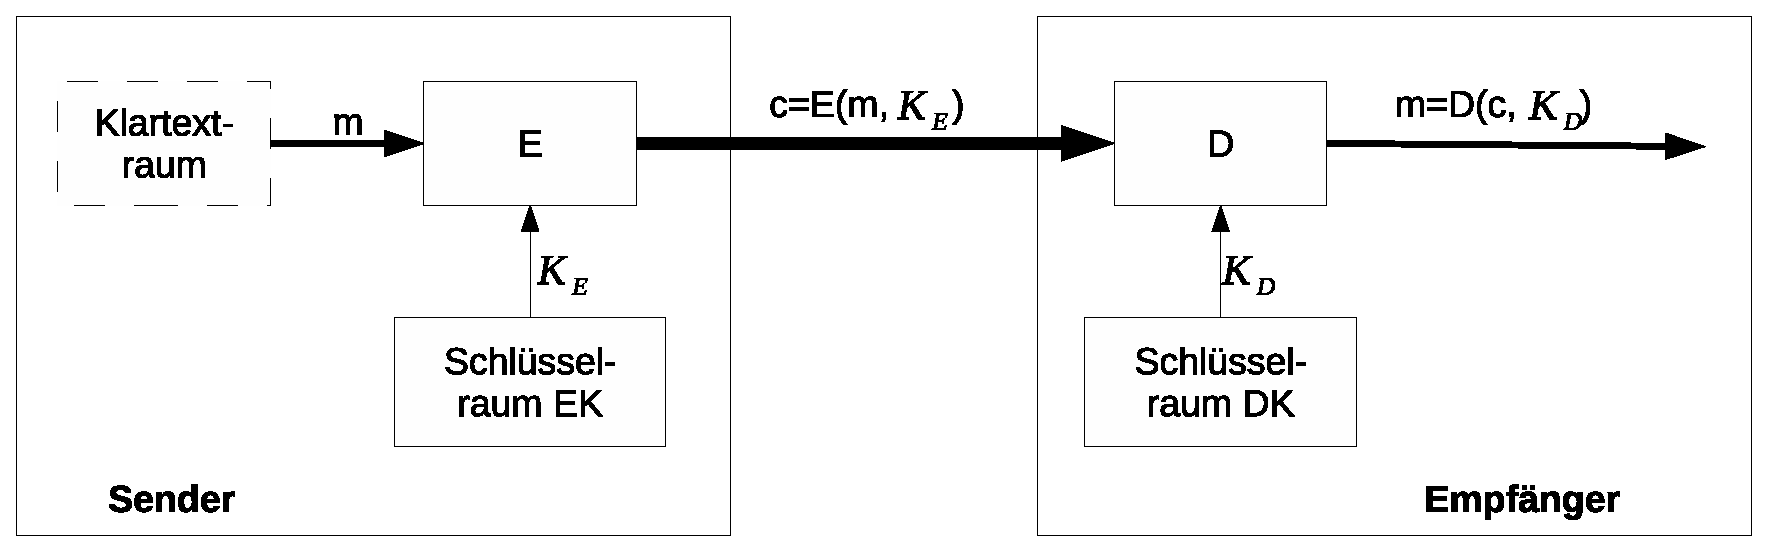
\includegraphics[width=\textwidth]{async.eps}
	\caption{Komponenten eines Kryptosystems}
	\label{fig:sim}
\end{figure}
\begin{multicols}{2}
\begin{enumerate}
\item Tupel \\($M,C,EK,DK,E,D$)
\item 2 endliche Alphabete \\($A_1,A_2$)
\item Menge von Klartexten \\($M \subseteq A^*_1\backslash\emptyset$)
\item Klartext \\($m \in M$)
\item Menge von Kryptotexten \\($C \subseteq A^*_2\backslash\emptyset$)
\item Kryptotext \\($c \in C$)
\item Verschlüsselungsschlüsselraum \\($EK\backslash\emptyset$)
\item Entschlüsselungsschlüsselraum\\($DK/\emptyset \\mit~ f:EK \rightarrow DK \\und~ f(K_E)=K_D)$
\item Verschlüsselungsverfahren \\($E :~ M x EK \rightarrow C$)
\item Entschlüsselungsverfahren \\($D :~ C x DK \rightarrow M$)
\item Es gilt: \\ $\forall m \in M : D(E(m,K_E),K_D) = m$
\end{enumerate}
\end{multicols}
Die Eigenschaft (11.) der obigen Legende zeigt uns das Zusammenspiel unserer einzelnen Komponenten. Wird ein Klartext m mit einem Schlüssel $K_E \in EK$ durch ein kryptographisches Verfahren E in einen Kryptotext umgewandelt. So ist gegeben, dass dieser Kryptotext unter Verwendung des zu $K_E$ gehörigen Schlüssels $K_D \in DK$, und des kryptographischen Verfahrens D wieder in den ursprünglichen Klartext m umgewandelt werden kann. Damit dies gegeben ist, muss unser asymmetrisches Kryptosystem einige wichtige Punkte erfüllen.
Es muss (nach ~\cite{Eckert13} ):
\newpage
\begin{enumerate}
\item eine effiziente Möglichkeit zur Erzeugung von Schlüsselpaaren ($K_E,K_D$) geben.
\item garantiert sein, dass der Private ($K_D$) nicht effizient aus dem öffentlichen Schlüssel ($K_E$) gebildet werden kann.
\item möglich sein effizient zu Ver- und Entschlüsseln.
\item optional aber nicht notwendiger Weise die Möglichkeit bestehen mit beiden Schlüsselpaaren zu verschlüsseln und mit dem jeweils anderem das Resultat zu entschlüsseln. Somit ist das System für Certifikate geiegnet.
\end{enumerate}

Um dies zu erreichen nutzen wir Einwegfunktionen.
%\subsection{Anwendung asymmetrischer Systeme}
\paragraph{Einwegfunktionen}
 sind besondere Funktionen ($f: X \rightarrow Y$) bei denen das Urbild ($X$) nicht unter vertretbarem zeitlichem Aufwand aus dem Bild ($Y$) zu berechnen ist. Mathematische Probleme, welche derartige Funktionen bilden, sind unter Anderem das Faktorisierungsproblem und der diskrete Algorithmus. Es ist nicht bewiesen, dass die Umkehrung nicht möglich ist, jedoch übersteigt die Komplexität der Berechnung unser heutiges Vermögen diese in einer vertretbaren Zeitspanne zu lösen.

\ \\
Bei der Verwendung von normalen Einwegfunktionen in einem Kryptosystem wäre zwar die Sicherheit der Daten garantiert, jedoch stellt die Umkehrung selbst für autorisierte Personen ein unüberwindbares Hindernis dar. Wir benötigen zum Entschlüsseln unserer Daten eine Hintertür - die so genannte Falltür. Einwegfunktionen mit Falltür bieten eine identische Sicherheit wie normale Einwegfunktionen, und die Option verschlüsselte Daten unter Kenntnis eines Geheimnisses (bei und der private oder öffentliche Schlüssel) zu entschlüsseln. Beispiele für mathematische Probleme mit Falltür sind die h-te Potenz modulo(n) und der zusammengesetzte Modul(n) (~\cite{Eckert13}). 

\subsection{RSA}
Bei RSA handelt es sich um ein 1978 von Ronald Rivest, Adi Shamir und Leonard Adleman entwickeltes Verfahren (~\cite{Eckert13}), welches   alle vier von uns genannten Bedingungen für ein asymmetrisches Kryptosystem erfüllt. Es beruht auf dem Faktorisierungsproblem.

\subsubsection{Schlüsselberechnung}
Zur Berechnung unseres Schlüsselpaares mit dem öffentlichen Schlüssel ($e,n$) und dem privaten Schlüssel ($d,\varphi(n)$) durchläuft man folgende Schritte:
\begin{enumerate}
\item Wähle zwei zufällige und große Primzahlen $p\neq q$.
\item Ermittle $n = p \cdot q$ und $\varphi(n) = (p-1)(q-1)$.
\item Wähle eine Zahl $e$ für die gilt: $ggt\Big(e,\varphi(n)\Big)$ und $1<e<\varphi(n)$
\item Als nächstes berechne $d$ mit $ed = 1 mod \varphi(n)$.
\item ($n,d$) ist der private Schlüssel, ($n,e$) ist der öffentliche Schlüssel
\end{enumerate} 

\subsubsection{Verschlüsselung und Entschlüsselung}
Möchten wir nun einen Klartext in einen Kryptotext umwandeln, haben wir zwei Schritte zu befolgen. Zunächst muss der Klartext ($m$) in eine Folge von Zahlen mit $m_i \in \{0,1,...,n-1\}$ umgewandelt werden. Daraufhin wird für alle $m_i~~~c_i=m^e_i mod n$ mit Hilfe des vorher berechneten öffentlichen Schlüssels bestimmt und wir erhalten den Kryptotext $c$. %~\cite{Schnor}
Die Umkehrung erfolgt ähnlich. Jedoch nutzen wir diesmal den privaten Schlüssel ($d,n$). Zuerst wird der Kryptotext in die Zahlenfolge umgewandelt indem wir $m_i = c^d_i mod n$ für alle $c_i$ bestimmen. Im Anschluss muss lediglich die Zahlenfolge wieder in unseren Klartext transformiert werden.
\ \\

Die Möglichkeit dieses Verfahren auch invers anzuwenden, ergo das Verschlüsseln mit dem privaten und das Entschlüsseln mit dem öffentlichen Schlüssel, wird bei Zertifikaten und E-Mail-Signaturen in Anspruch genommen. Bei letzterem wird aus dem Inhalt der E-Mail ein Hashcode generiert, welcher mit dem privaten Schlüssel verschlüsselt als Signatur an die Nachricht angehangen und dann verschickt wird. Dabei geht es weniger um das Geheimhalten des Inhaltes der Nachricht, Sondern um das Sicherstellen, dass sie unverfälscht beim Empfänger eintrifft. Nach Erhalt der E-Mail kann der Empfänger die Signatur mit dem öffentlichen Schlüssel des Senders entschlüsseln und den Inhalt der Nachricht mit dem Hashcode abgleichen. Sollte es dabei zu Unstimmigkeiten kommen ,ist bewiesen, dass die Nachricht nach Anhängen der Signatur verändert wurde.


\subsection{Schlüsselmanagement}
Bei der asymmetrischen Kryptographie ergeben sich aufgrund ihrer besonderen Grundidee der zwei Schlüssel auch ganz eigene Möglichkeiten und Pflichten zur Erzeugung, Aufbewahrung und möglichen Wiederherstellung dieser. 

\paragraph{Die Erzeugung}
asymmetrischen Schlüsselmaterials kann der Nutzer entweder selbst übernehmen oder einer zentralen Instanz (z.B. CA) überlassen.
Sollte der Nutzer den Schlüssel selbst generieren, hat dies zum Vorteil, dass er die volle Kontrolle über den Erstellungsprozess besitzt. Jedoch obliegt ihm somit auch die Verantwortung den Prozess und die fertigen Schlüssel durch nötige Einstellungen im System und nötige Vorsicht zu sichern. Besonderes Augenmerk liegt dabei auf dem privaten Schlüssel, welcher unter keinen Umständen öffentlich werden darf. Da die Sicherheit der verschlüsselten Daten dann nicht mehr gewährleistet ist. 
Im Falle der Erzeugung durch eine zentrale Instanz gibt der Nutzer diese Verantwortung größtenteils aus der Hand. Dabei sollte er sich jedoch bewusst sein, dass so auch keine Kontrolle seinerseits besteht. Des Weiteren ist es nun notwendig den privaten Schlüssel sicher dem Nutzer zur Verfügung zu stellen, was unter Umständen kritisch werden kann. Ist der Schlüssel erstmal erzeugt, muss dieser zwingend sicher aufbewahrt werden.

\paragraph{Die Schlüsselspeicherung}
muss gewährleisten, dass der private Schlüssel keinem Unbefugten zur Verfügung steht. Um ein Fehlverhalten des Nutzers auszuschließen, wäre es also ratsam nicht einmal diesem den Zugang zu dem privaten Schlüssel zu gestatten. Diesen Weg gehen Token (oder SmartCard). Token sind Chipkarten oder USBsticks bei denen der Schlüssel auf einem internen Chip sicher verwahrt wird. Der Zugriff ist ausschließlich über Sicherheitssoftware in Emailprogrammen (PGP) oder anderen (OpenSSH) möglich, welche den Schlüssel selbstständig auslesen und ihn nicht zwischenspeichern. Außerdem ist es natürlich möglich den Schlüssel selbst sicher zu verwahren.

\paragraph{Die Verbreitung}
des öffentlich Schlüssels ist über beliebige Wege möglich. Zum Einen besteht die Möglichkeit den öffentlichen Schlüssel auf einem KeyServer zu lagern oder ihn per E-Mail zu verschicken. Es gibt noch wesentlich mehr Alternativen zur Verbreitung, welche hier nicht alle genannt werden sollen. Allerdings ist die Authentizität des öffentlich Schlüssels zu berücksichtigen.Denn nicht immer lässt sich garantieren das der Schlüssel den man als öffentlichen Schlüssel von Person A gefunden oder erhalten hat auch wirklich von dieser stammt. Zu diesem Zweck werden Schlüssel von Gesprächspartnern, welche sich bereits gegenseitig überprüft haben, unterschrieben. Somit bestätigt der Signierende die Zugehörigkeit des öffentlichen Schlüssels zu Person A. Es wird eine mit dem privaten Schlüssel des Signierenden verschlüsselte Signatur an den öffentlichen Schlüssel von Person A angehangen. Aufgrund dessen unsere Operationen umkehrbar sind. Lässt sich nun diese Signatur mit dem öffentlichen Schlüssel des Unterzeichners öffnen und überprüfen. Da die Signatur jedoch nicht geändert werden kann, ist sie zudem vor Fälschung sicher. Dieses Verfahren wird ebenso bei Certifikaten im WebOfTrust oder wie bereits erwähnt beim E-Mail Verkehr genutzt.

\subsection{Hybride Kryptographie}


\section{Kryptographie mit Java}
\subsection{Java Cryptography Architecture}

\subsection{Zufallszahlen}

\subsection{Schlüsselgenerierung}

\subsection{Schlüsselspeicherung}

\subsection{Schlüsseleinigung}

\subsection{Ver- und Entschlüsselung}

\section{Zusammenfassung}
Zum Schluss bitte eine Zusammenfassung!

\bibliographystyle{alpha}
\bibliography{lit}

\end{document}
